\documentclass[11pt,a4paper]{article}
\usepackage[utf8]{inputenc}
\usepackage[T1]{fontenc}
\usepackage{lmodern}
\usepackage[margin=2.4cm,headheight=15pt]{geometry}
\usepackage{xcolor,booktabs,array,tabularx,longtable,enumitem,graphicx,listings,fancyhdr,hyperref,tikz}
\usetikzlibrary{arrows.meta,positioning,fit,shapes.geometric}
\definecolor{navy}{HTML}{18354B}
\definecolor{bluebg}{HTML}{EAF2FA}
\hypersetup{colorlinks=true,linkcolor=navy,urlcolor=navy,pdftitle={Laporan UTS EventKu Kelompok IV}}
\pagestyle{fancy}\fancyhf{}\fancyhead[L]{\small EventKu -- Laporan UTS}\fancyhead[R]{\small Kelompok IV}\fancyfoot[C]{\thepage}
\setlength{\parindent}{0pt}\setlength{\parskip}{7pt}
\renewcommand{\contentsname}{Daftar Isi}
\setlist{nosep,leftmargin=*,topsep=4pt}
\renewcommand{\arraystretch}{1.2}
\newcolumntype{Y}{>{\raggedright\arraybackslash}X}
\newcommand{\tbl}[2]{\par\smallskip\noindent\begin{tabularx}{\linewidth}{#1}\toprule #2\bottomrule\end{tabularx}\par\smallskip}
\newcommand{\note}[1]{\par\smallskip\noindent\fcolorbox{navy}{bluebg}{\parbox{\dimexpr\linewidth-2\fboxsep-2\fboxrule\relax}{\small #1}}\par\smallskip}
\newcommand{\page}[1]{\clearpage\section{#1}}
\tikzset{box/.style={draw=navy,rounded corners,fill=bluebg,align=center,text width=3cm,minimum height=1cm,font=\small},arr/.style={-{Stealth},draw=navy},uc/.style={ellipse,draw=navy,fill=bluebg,align=center,text width=3cm,minimum height=.9cm,font=\small}}
\lstset{basicstyle=\ttfamily\small,breaklines=true,frame=single,backgroundcolor=\color{bluebg},columns=fullflexible,keepspaces=true,showstringspaces=false}
\newcommand{\lucidfig}[3]{\par\begin{center}\includegraphics[width=\linewidth,height=#2,keepaspectratio]{figures/#1.png}\par\small #3\par\footnotesize Sumber: ekspor Lucidchart versi revisi dalam DOCX kelompok. \href{https://lucid.app/lucidchart/c1ed1ac4-eabd-423c-a2b8-d558d07f165d/edit}{Buka dokumen Lucidchart}.\end{center}\par}
\newcommand{\uifig}[3]{\par\begin{center}\includegraphics[width=\linewidth,height=#2,keepaspectratio]{figures/figma/#1.png}\par\small #3\par\footnotesize Sumber: rancangan Figma Audrey, pada DOCX wireframe dan UI high-fidelity Minggu 7.\end{center}\par}
\begin{document}
\begin{titlepage}\centering
{\Large Universitas Katolik Widya Mandala Surabaya\par}
{\large Fakultas Teknik -- Program Studi Informatika\par}
\vspace{1.5cm}{\Huge\bfseries\color{navy} EventKu\par}
\vspace{.5cm}{\LARGE Laporan Ujian Tengah Semester\par}
{\large INF300 -- Rekayasa Perangkat Lunak\par}
{\large Semester Gasal 2026/2027\par}
\vspace{1cm}{\large Sistem Informasi dan Pendaftaran Event Kampus\par}
\vspace{1cm}\begin{tabular}{ll}
Audrey Elizabeth Gracesia & 5803024014\\
Bambang Herlambang & 5803024019\\
Dustin Pranata Wangsawidjaja & 5803024021\\
Alexa Bilxiz Aulia & 5803024023\\
\end{tabular}\par\vspace{.7cm}Kelompok IV
\vfill\note{Draf laporan berdasarkan artefak proyek sampai 7 Oktober 2026. Konfirmasi kondisi aktual tim dan jawaban individu bagian C--D masih harus dilengkapi sebelum pengumpulan.}
\vspace{.5cm}Surabaya, 7 Oktober 2026
\end{titlepage}
\tableofcontents
\page{Identitas dan Deskripsi Proyek}
EventKu adalah aplikasi web untuk memusatkan informasi kegiatan kampus dan pendaftaran peserta. Laporan ini menggabungkan analisis kebutuhan dan rancangan kelompok sampai tahap UTS. SRS versi 2 menjadi acuan kebutuhan; Figma merupakan artefak visual yang belum mencakup seluruh kebutuhan.
\subsection{Pembagian Peran}
\tbl{p{3.6cm}p{3cm}Y}{Nama & Peran & Tanggung jawab\\\midrule
Audrey Elizabeth Gracesia & Backend dan UI/UX & Rancangan API, alur backend, wireframe dan antarmuka.\\
Bambang Herlambang & System Architect dan Frontend & ERD, arsitektur modular, class diagram, pattern dan frontend.\\
Dustin Pranata Wangsawidjaja & PM dan Business Analyst & Charter, SDLC, SRS, backlog dan koordinasi.\\
Alexa Bilxiz Aulia & QA dan DevOps & Rancangan pengujian, kualitas, kolaborasi dan deployment.\\}
\subsection{Latar Belakang}
Informasi seminar, lomba, workshop, dan kegiatan organisasi tersebar melalui poster, grup percakapan, dan media sosial. Mahasiswa perlu memeriksa banyak saluran untuk mengetahui jadwal, lokasi, serta pendaftaran. Penyelenggara membutuhkan pencatatan peserta yang konsisten dengan kapasitas kegiatan.
Pemusatan informasi membantu mahasiswa menemukan kegiatan sesuai minat dan membantu penyelenggara memantau peserta. Moderasi admin diperlukan agar katalog publik hanya menampilkan kegiatan yang disetujui.
\subsection{Masalah Utama}
\begin{itemize}
\item Informasi kegiatan sulit ditelusuri berdasarkan jadwal atau kategori.
\item Pendaftaran terpisah dari informasi dan berisiko duplikasi atau melebihi kuota.
\item Penyelenggara memerlukan status publikasi, daftar peserta, dan ekspor data.
\item Pengelolaan organisasi dan publikasi memerlukan aturan akses yang jelas.
\end{itemize}
\page{Tujuan, Ruang Lingkup, dan Batasan}
\tbl{p{4cm}Y}{Tujuan & Bukti keberhasilan yang perlu diperoleh\\\midrule
Memudahkan pencarian & Kata kunci, kategori, tanggal, penyelenggara menghasilkan daftar event Disetujui.\\
Menertibkan pendaftaran & Satu pendaftaran aktif per mahasiswa per event; kuota tidak terlampaui pada permintaan bersamaan.\\
Menjaga kualitas publikasi & Event melewati pengajuan dan moderasi; penolakan memuat alasan.\\
Membantu penyelenggara & Peserta dan ekspor CSV sesuai lingkup organisasi serta hak akses.\\
Memudahkan penggunaan & Responsif minimal 360 piksel, bahasa Indonesia; pencarian--RSVP ditargetkan maksimal lima klik.\\}
\subsection{Lingkup MVP}
\begin{enumerate}
\item Registrasi, login, logout, JWT, dan otorisasi mahasiswa, penyelenggara, admin.
\item Verifikasi organisasi sebelum pengajuan kegiatan.
\item Draft, pengajuan, moderasi, pengelolaan event dan katalog publik.
\item Pencarian, filter gabungan, detail dan kalender bulanan.
\item RSVP, pembatalan sebelum mulai, riwayat dan kontrol kuota atomik.
\item Minat kategori, daftar notifikasi dan pemberitahuan event baru.
\item Dashboard, daftar peserta, ekspor CSV dan pengelolaan kategori.
\end{enumerate}
\subsection{Batasan}
Aplikasi native, tiket berbayar, dan integrasi SSO kampus berada di luar MVP. Bookmark, rating, dan beberapa notifikasi tambahan mengikuti prioritas Should/Could serta kapasitas tim. Proyek berlangsung 16 minggu dengan empat anggota. Data demonstrasi perlu disiapkan sebagai data uji.
Laporan ini tidak menyatakan sistem telah berjalan di produksi atau target performa telah tercapai. PostgreSQL ditetapkan sebagai database relasional. Persetujuan pemangku kepentingan dan hasil pengujian aktual tetap perlu dikonfirmasi tim.
\page{SDLC dan Posisi Proyek}
\subsection{Scrum yang Diadaptasi untuk Perkuliahan}
Dokumen justifikasi memilih Scrum karena kebutuhan dapat berkembang, risiko integrasi perlu diketahui lebih awal, dan implementasi dapat dibagi menjadi increment. Tim memakai backlog MoSCoW dan merencanakan planning, review, serta retrospective.
Analisis dan rancangan awal dilakukan sebelum UTS, sedangkan standup direncanakan mengikuti ketersediaan tim. Ini adaptasi untuk perkuliahan, bukan bukti bahwa seluruh praktik Scrum resmi sudah diterapkan. Scrum menggunakan pendekatan iteratif dan inkremental serta inspeksi dan adaptasi \cite{scrum}.
\begin{center}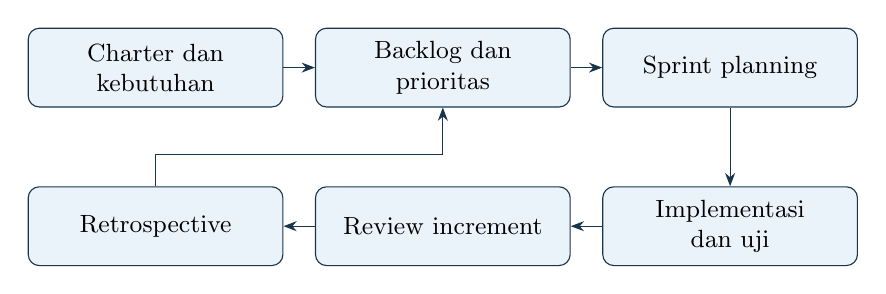
\begin{tikzpicture}[node distance=.4cm]
\node[box] (a) {Charter dan kebutuhan};\node[box,right=of a] (b) {Backlog dan prioritas};\node[box,right=of b] (c) {Sprint planning};
\node[box,below=1cm of c] (d) {Implementasi dan uji};\node[box,left=of d] (e) {Review increment};\node[box,left=of e] (f) {Retrospective};
\draw[arr] (a)--(b);\draw[arr] (b)--(c);\draw[arr] (c)--(d);\draw[arr] (d)--(e);\draw[arr] (e)--(f);\draw[arr] (f.north)--++(0,.4)-|(b.south);
\end{tikzpicture}\par\small Gambar 1. Siklus pengembangan yang direncanakan.\end{center}
\tbl{p{2.6cm}p{1.7cm}Y}{Tahap & Minggu & Artefak/rencana\\\midrule
Inisiasi & 1 & Identitas, masalah, peran, charter.\\
Analisis & 2--4 & SRS, user story, backlog dan prioritas.\\
Perancangan & 5--7 & Activity diagram, ERD, arsitektur, UML, Figma dan pattern.\\
Evaluasi UTS & 8 & Konsolidasi laporan dan evaluasi kesiapan.\\
Implementasi & 9--13 & Increment aplikasi dan pengujian tiap sprint.\\
Validasi akhir & 14--16 & Pengujian sistem, UAT, deployment, dokumentasi.\\}
Artefak rancangan tersedia; ketersediaannya tidak membuktikan review, persetujuan, atau implementasi fitur telah selesai.
\page{Perbandingan SDLC dan Pengendalian Iterasi}
Penilaian berikut berasal dari justifikasi internal tim. Skala 1--5 menunjukkan kesesuaian dengan konteks proyek, bukan pengukuran independen.
\tbl{Yrrrr}{Kriteria & Bobot & Waterfall & Iteratif & Scrum\\\midrule
Adaptasi perubahan & 5 & 1 & 4 & 5\\
Deteksi risiko dini & 5 & 2 & 4 & 5\\
Waktu 16 minggu & 4 & 3 & 3 & 4\\
Transparansi kemajuan & 4 & 3 & 3 & 5\\
Tim kecil & 3 & 3 & 4 & 5\\
Dokumentasi & 4 & 5 & 3 & 3\\
Kemudahan bagi pemula & 3 & 4 & 3 & 3\\\midrule
Total berbobot & 28 & 80 & 97 & 122\\}
\subsection{Kelebihan dan Keterbatasan}
Waterfall menyediakan urutan dan dokumentasi jelas, tetapi perubahan kebutuhan dapat memerlukan revisi lintas tahap. Model iteratif memungkinkan penyempurnaan bertahap; prioritas dan penilaian increment tetap diperlukan. Scrum mendukung transparansi backlog dan review rutin, tetapi memerlukan komitmen, kapasitas yang realistis, serta definisi selesai terukur.
\subsection{Pengendalian Perubahan}
Perubahan dicatat dengan ID kebutuhan, alasan, dampak pada diagram/API, dan estimasi. PM/BA mengelola prioritas bersama tim. Must didahulukan; Should/Could tidak boleh mengorbankan integritas kuota, otorisasi dan moderasi.
\note{Dokumen awal menyebut tiga sprint sekitar dua minggu pada Minggu 9--13, sedangkan rentang ini hanya lima minggu. Usulan konsisten: Sprint 1 Minggu 9--10, Sprint 2 Minggu 11--12, Sprint 3 Minggu 13. Ini perlu disepakati tim.}
Definition of Ready memastikan kebutuhan dan penerimaan dipahami. Definition of Done disarankan mencakup review kode, pengujian relevan, pembaruan dokumentasi/API, dan demonstrasi increment. Bukti pelaksanaannya baru dapat dilaporkan setelah aktivitas tersebut berlangsung.
\page{Pemangku Kepentingan dan Kebutuhan Fungsional}
\tbl{p{3cm}Yp{3.4cm}}{Pihak & Kebutuhan & Keterlibatan\\\midrule
Mahasiswa & Pencarian, RSVP, kalender, minat/notifikasi. & Pengguna dan calon peserta UAT.\\
Penyelenggara & Mengajukan event dan mengelola peserta organisasi sendiri. & Pemilik konten/validator alur.\\
Admin & Verifikasi, moderasi, kategori. & Pengendali publikasi.\\
Pengunjung & Informasi publik tanpa login. & Pengguna katalog.\\
Dosen & Artefak dan penerapan rekayasa perangkat lunak. & Evaluator perkuliahan.\\
Tim pengembang & Kebutuhan jelas, kontrak stabil, kualitas terukur. & Analisis, desain, implementasi, QA.\\}
\subsection{Kebutuhan Inti}
\tbl{p{3cm}Y}{ID & Ringkasan kebutuhan Must\\\midrule
FR-AUTH-01 & Registrasi nama, email, kata sandi dan peran.\\
FR-AUTH-04 & Otorisasi peran pada UI dan API.\\
FR-AUTH-05 & Verifikasi organisasi sebelum pengajuan event.\\
FR-EVT-01 & Event memuat waktu mulai/selesai, lokasi, poster, kategori dan kuota.\\
FR-EVT-03 & Status Draft, Menunggu Moderasi, Disetujui, Ditolak, Selesai, Dibatalkan.\\
FR-MOD-02 & Admin menyetujui/menolak dengan alasan penolakan.\\
FR-MOD-03 & Katalog dan kalender hanya memuat event Disetujui.\\
FR-SRC-02/03 & Kata kunci serta filter kategori, tanggal, penyelenggara.\\
FR-RSV-02 & Menolak pendaftaran penuh atau duplikasi aktif.\\
FR-RSV-03 & Pembatalan sebelum mulai mengembalikan kuota.\\
FR-RSV-06 & Kuota konsisten pada permintaan bersamaan.\\
FR-NTF-02 & Notifikasi event baru sesuai minat kategori.\\
FR-DSH-04 & Ekspor daftar peserta dalam CSV.\\}
Daftar lengkap dan prioritas terdapat pada lampiran. Must merupakan lingkup wajib; Should dan Could tetap dibedakan dalam implementasi dan pengujian.
\page{Kebutuhan Nonfungsional dan Verifikasi}
\tbl{p{2.9cm}Yp{4cm}}{ID & Target rancangan & Verifikasi yang direncanakan\\\midrule
NFR-PERF-01 & Home/daftar termuat dalam 3 detik pada 4G standar. & Catat perangkat, dataset, jaringan, cache dan waktu muat.\\
NFR-PERF-02 & Sekitar 95\% API baca $\leq$500 ms; tulis $\leq$1 s pada beban normal. & Uji beban; definisikan beban normal dan ukur persentil.\\
NFR-PERF-03 & 100 pengguna bersamaan (Should). & Konkurensi, error rate, latensi.\\
NFR-SEC-01/02 & Hash kata sandi, JWT kedaluwarsa, HTTPS produksi. & Review konfigurasi dan uji token.\\
NFR-SEC-03 & Peran/kepemilikan diperiksa server. & Uji negatif lintas akun/organisasi.\\
NFR-SEC-04 & Validasi input, mitigasi SQLi/XSS. & Query berparameter, validasi payload, uji input berbahaya.\\
NFR-MOD-01/02 & Empat modul; repository mengakses data. & Review kontrak dan dependensi.\\
NFR-MOD-04 & Observer tanpa pemanggilan langsung layanan notifikasi. & Uji handler/event sesudah commit.\\
NFR-SCAL-03 & Pagination dan indeks pencarian. & Review query/execution plan.\\
NFR-USA-01 & Responsif minimal 360 piksel. & Pemeriksaan desktop dan mobile.\\
NFR-MAINT-02 & Coverage inti Auth/Event minimal 60\% (Should). & Laporan coverage ketika kode tersedia.\\
NFR-REL-01 & Availability 99\% saat demo/UAT, di luar pemeliharaan (Should). & Log pada periode yang ditetapkan.\\}
Target berasal dari SRS dan belum merupakan hasil pengukuran. Pengujian harus mencantumkan versi aplikasi, lingkungan, data, langkah, hasil dan status. Artefak testcase menunjukkan persiapan; laporan ini tidak menyimpulkan semuanya telah dijalankan atau lulus.
\page{Model Use Case}
Diagram berikut digambar ulang dalam LaTeX berdasarkan SRS, bukan diambil dari Lucidchart. Diagram menampilkan interaksi utama; daftar lengkap tersedia pada lampiran. Proses otomatis memakai aktor penjadwal.
\begin{center}\resizebox{\linewidth}{!}{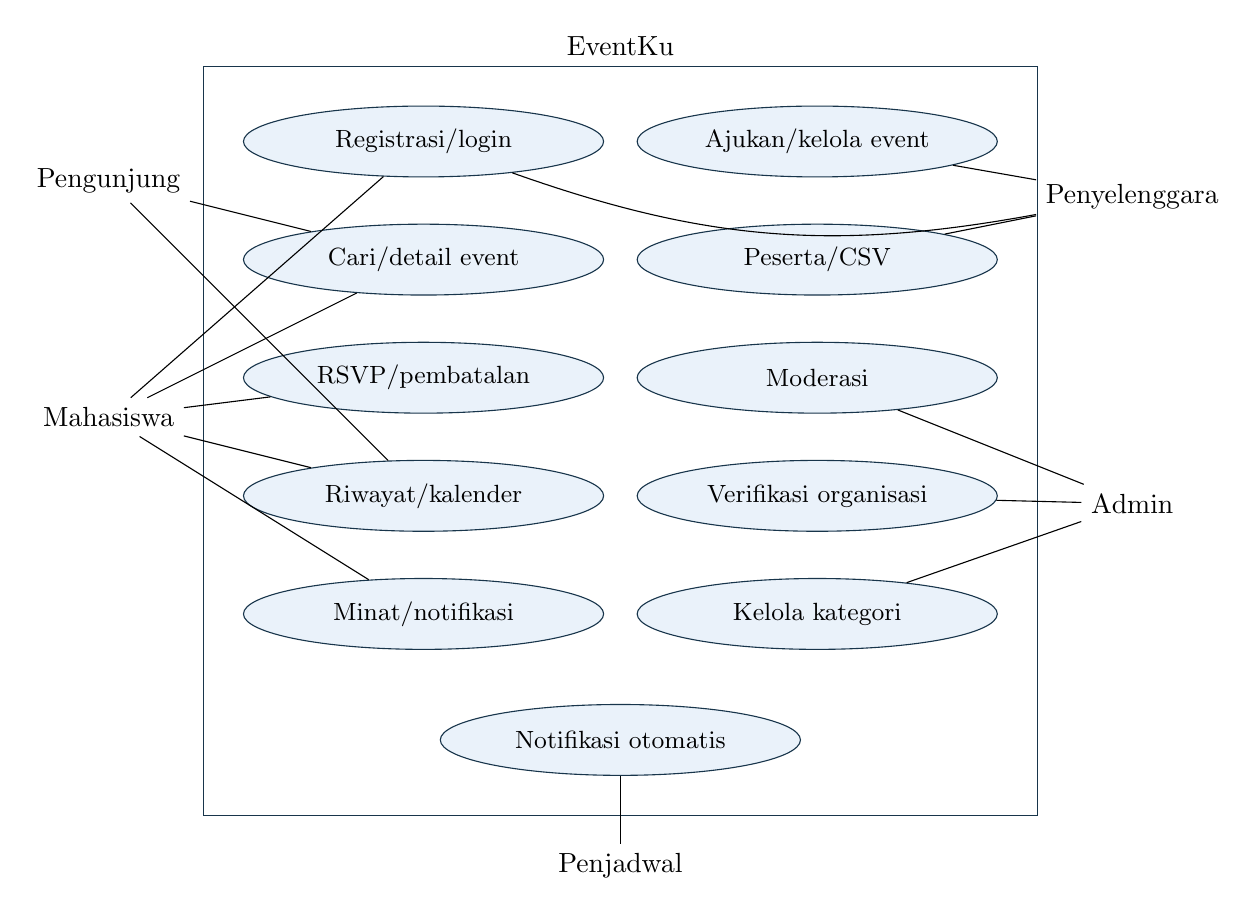
\begin{tikzpicture}
\node[uc] (u1) at (0,0) {Registrasi/login};\node[uc] (u2) at (0,-1.5) {Cari/detail event};\node[uc] (u3) at (0,-3) {RSVP/pembatalan};\node[uc] (u4) at (0,-4.5) {Riwayat/kalender};\node[uc] (u5) at (0,-6) {Minat/notifikasi};
\node[uc] (u6) at (5,0) {Ajukan/kelola event};\node[uc] (u7) at (5,-1.5) {Peserta/CSV};\node[uc] (u8) at (5,-3) {Moderasi};\node[uc] (u9) at (5,-4.5) {Verifikasi organisasi};\node[uc] (u10) at (5,-6) {Kelola kategori};\node[uc] (u11) at (2.5,-7.6) {Notifikasi otomatis};
\node[draw=navy,fit=(u1)(u6)(u11),inner sep=.5cm,label=above:EventKu] {};
\node (g) at (-4,-.5) {Pengunjung};\node (s) at (-4,-3.5) {Mahasiswa};\node (o) at (9,-.7) {Penyelenggara};\node (a) at (9,-4.6) {Admin};\node (p) at (2.5,-9.2) {Penjadwal};
\draw (g)--(u2);\draw (g)--(u4);\foreach \u in {u1,u2,u3,u4,u5}\draw (s)--(\u);
\draw (o)--(u6);\draw (o)--(u7);\draw (o) to[bend left=15] (u1);\foreach \u in {u8,u9,u10}\draw (a)--(\u);\draw (p)--(u11);
\end{tikzpicture}}\par\small Gambar 2. Diagram digambar ulang dalam LaTeX berdasarkan SRS versi 2; bukan ekspor Lucidchart.\end{center}
Pengunjung mengakses katalog publik; mahasiswa mengelola pendaftaran dan notifikasi sendiri. Penyelenggara mengelola event serta peserta dalam lingkup organisasi yang diizinkan. Admin menjalankan verifikasi/moderasi. Backend tetap memeriksa semua izin walaupun UI telah membatasi menu.
\page{Deskripsi Use Case: RSVP}
\tbl{p{3cm}Y}{Elemen & UC-05 -- Mendaftar event\\\midrule
Aktor & Mahasiswa.\\
Tujuan & Satu pendaftaran aktif pada kegiatan pilihan.\\
Prakondisi & Login; event Disetujui, belum berakhir, memiliki kursi tersedia.\\
Pemicu & Tombol RSVP pada detail event.\\
Alur utama & (1) UI mengirim ID event; (2) server mengambil identitas JWT; (3) periksa status/waktu; (4) transaksi memeriksa pendaftaran dan mereservasi kursi; (5) simpan/aktifkan pendaftaran; (6) commit; (7) kirim hasil; (8) publikasikan StudentRegistered.\\
Alternatif & Token tidak valid: login kembali. Penuh: tolak tanpa perubahan. Sudah aktif: tidak menambah kursi. Pernah dibatalkan: aktifkan ulang jika memenuhi syarat. Operasi gagal: rollback seluruh perubahan.\\
Pascakondisi & Satu pendaftaran aktif; penghitung bertambah satu dan tidak melebihi kuota.\\
Kebutuhan & FR-RSV-01,02,06; konfirmasi in-app FR-RSV-05 adalah Should.\\}
\subsection{Pembatalan}
Mahasiswa hanya membatalkan pendaftaran sendiri sebelum waktu mulai. Perubahan status dan pengembalian kursi berada dalam satu transaksi. Permintaan pembatalan ulang tidak mengurangi penghitung lagi. Riwayat tetap tersedia.
\subsection{Skenario Penerimaan}
\begin{enumerate}
\item Dua permintaan kursi terakhir: hanya satu berhasil.
\item Permintaan ulang pendaftaran aktif: tidak membuat rekaman/reservasi baru.
\item Gagal menyimpan sesudah reservasi: rollback mengembalikan penghitung.
\item Pembatalan lintas akun atau sesudah mulai: ditolak tanpa perubahan.
\end{enumerate}
Skenario di atas adalah rencana validasi, bukan hasil uji aktual.
\page{Deskripsi Use Case: Pengajuan dan Moderasi}
\tbl{p{2.6cm}Y}{Elemen & UC-10 -- Mengajukan event\\\midrule
Aktor/tujuan & Penyelenggara; meminta persetujuan publikasi.\\
Prakondisi & Login, organisasi terverifikasi, memiliki hak terhadap draft.\\
Alur utama & Isi judul, deskripsi, kategori, mulai/selesai, lokasi/tautan, poster dan kuota. Server memvalidasi. Simpan Draft lalu ajukan menjadi Menunggu Moderasi.\\
Alternatif & Data salah, akhir tidak sesudah mulai, organisasi belum terverifikasi, atau draft pihak lain: ditolak dengan alasan yang sesuai.\\
Pascakondisi & Masuk antrean admin, belum menjadi katalog publik.\\
Kebutuhan & FR-AUTH-05; FR-EVT-01--05.\\}
\vspace{.4cm}
\tbl{p{2.6cm}Y}{Elemen & UC-13 -- Moderasi event\\\midrule
Aktor/tujuan & Admin; memutuskan kelayakan publikasi.\\
Prakondisi & Login admin; event Menunggu Moderasi.\\
Alur utama & Buka antrean/detail. Setujui atau tolak dengan alasan. Server memeriksa transisi, menyimpan keputusan, commit, mempublikasikan EventModerated; persetujuan juga mempublikasikan EventApproved.\\
Alternatif & Alasan kosong: minta perbaikan. Status berubah: tolak transisi/muat ulang. Token atau peran salah: tolak akses.\\
Pascakondisi & Disetujui atau Ditolak; hasil in-app untuk penyelenggara. Persetujuan membuka katalog dan notifikasi minat.\\
Kebutuhan & FR-MOD-01--04; riwayat FR-MOD-06 adalah Should.\\}
Versi keputusan mencegah notifikasi moderasi berikutnya hilang karena deduplikasi terlalu umum. Edit penting setelah persetujuan memerlukan moderasi ulang jika fitur Should tersebut diimplementasikan.
\page{Arsitektur Sistem}
\subsection{Modular Monolith}
Satu backend Express.js memiliki empat modul. Pilihan ini mengurangi beban operasional tim kecil dan memungkinkan transaksi database bersama, sekaligus menjaga batas tanggung jawab. Frontend React/Tailwind berkomunikasi melalui HTTP/JSON.
\lucidfig{arsitektur_modular}{.48\textheight}{Gambar 3. Arsitektur modular EventKu (ekspor Lucidchart).}
\note{Database yang dipilih adalah PostgreSQL, sesuai konfirmasi Bambang dan README yang menggunakan Neon PostgreSQL. Rencana hosting tetap Vercel untuk frontend dan Render untuk backend. Pilihan tipe ID UUID/BIGINT masih perlu ditetapkan sebelum migrasi dibuat.}

\page{Rancangan Antarmuka Figma}
Rancangan UI dibuat Audrey pada Minggu 7 dan digunakan sebagai acuan visual awal. Sembilan tampilan yang tersedia mencakup Home, Login, Register, Dashboard Mahasiswa, Detail Event, Calendar, Kelola Event, Tambah Event dan Edit Event. Gambar diambil tanpa mengubah isi dari dokumen UI kelompok.
\subsection{Home dan Pencarian}
Home menampilkan navigasi, kata kunci, kategori dan kartu event mendatang. Tampilan ini mendukung alur pencarian dan pembukaan detail kegiatan (UC-03 dan UC-04).
\uifig{home}{.50\textheight}{Gambar UI-1. Home EventKu pada rancangan Figma.}
\href{https://www.figma.com/design/msefrhl4aO32NFpVU4MRlo/RPL-EventKu--UTS-}{Buka desain Figma}\quad\href{https://www.figma.com/proto/msefrhl4aO32NFpVU4MRlo/RPL-EventKu--UTS-?node-id=1-52}{Buka prototype Figma}.
\note{Mockup merupakan rancangan visual, bukan bukti implementasi atau seluruh kebutuhan SRS sudah tercakup. Hak akses dan status tetap mengikuti SRS versi 2.}
\clearpage\subsection{Detail Event dan RSVP}
Detail event menampilkan poster, jadwal, lokasi, penyelenggara, kuota, deskripsi dan tombol daftar. Alur ini mendukung UC-04 dan UC-05. Tombol Simpan Event pada mockup merupakan fitur bookmark berprioritas Could, sehingga bukan lingkup wajib MVP.
\uifig{detail_event}{.53\textheight}{Gambar UI-2. Detail event dan tombol pendaftaran pada Figma.}
\subsection{Cakupan dan Penyesuaian saat Implementasi}
Dashboard mahasiswa, kalender dan halaman pengelolaan tersedia pada lampiran. Label Admin/Campus dan Dipublikasikan pada mockup dipertahankan sebagai bukti desain awal. Implementasi memakai pembagian hak akses penyelenggara terverifikasi dan admin serta enam status yang ditentukan SRS. Form waktu mulai/selesai, moderasi, minat/notifikasi, dan tampilan mobile perlu dirinci mengikuti SRS tanpa menganggap semua sudah tergambar.
\page{Tanggung Jawab dan Aliran Data}
\tbl{p{3cm}Y}{Komponen & Tanggung jawab\\\midrule
View React & Form, hasil, loading/error dan navigasi; tidak menetapkan izin server.\\
Hooks/API client & Aksi UI, validasi awal, permintaan HTTP dan pembaruan data halaman.\\
Context & State sesi/peran/organisasi bersama; bukan pengganti aturan bisnis.\\
Controller & Request, aktor terverifikasi, pemanggilan service, HTTP/DTO.\\
Service/domain & Aturan bisnis, transisi status, kepemilikan dan transaksi.\\
Repository & SQL berparameter, filter, pagination, kontrak yang dapat diuji.\\
Facade publik & Akses lintas modul tanpa mengimpor repository privat.\\
EventBus/handler & Event setelah commit; pemilihan penerima notifikasi.\\}
\subsection{Aliran Pencarian}
View mengirim GET /api/v1/events. Controller dan service menormalisasi query serta menetapkan lingkup publik Disetujui. Repository menggunakan filter identik untuk count dan daftar, dengan urutan stabil. Controller mengirim JSON; UI menampilkan hasil atau keadaan kosong.
\subsection{Modularitas dan Kualitas}
Kontrak publik menjaga batas modul; pemisahan UI, bisnis dan SQL membantu pemeliharaan. Pagination, indeks dan backend stateless mendukung skalabilitas awal. Pada peningkatan pengguna sepuluh kali, ukur query pencarian, koneksi database, serta kontensi kuota sebelum memilih caching atau pemisahan layanan.
EventBus in-process sesuai tahap awal, tetapi kegagalan proses setelah commit dapat melewatkan notifikasi. Outbox, worker, retry dan handler idempoten dapat dipertimbangkan jika diperlukan keandalan pengiriman lebih tinggi.
\subsection{Kontrak API Awal}
Kelompok endpoint meliputi auth/register, auth/login, events, pengajuan/moderasi, registrations, notifications, organisasi dan kategori. Identitas diambil dari JWT, bukan ID aktor bebas dari request. Respons membedakan 401 autentikasi, 403 izin, 404 data hilang, 409 konflik kuota/status/duplikasi, serta 422 input tidak valid.
\page{Rancangan Modul dan Struktur Data}
\subsection{Auth}
\tbl{p{2.7cm}Y}{Aspek & Rancangan\\\midrule
Tujuan & Akun, autentikasi dan identitas aktor.\\
Input & Nama, email, kata sandi, peran publik; kredensial login.\\
Proses & Validasi, email unik, hash, simpan; login memverifikasi hash dan menghasilkan JWT.\\
Output & UserDTO tanpa hash; token memiliki masa berlaku.\\
Dependensi & UserRepository, hash provider, JwtProvider, status organisasi.\\
Struktur data & User, Organization, claims; email unik dan peran terbatas.\\}
Admin tidak dibuat melalui signup publik. Status verifikasi diperiksa server. Strategi penyimpanan token perlu ditetapkan dengan mempertimbangkan risiko XSS dan kebutuhan sesi.
\subsection{Event dan Pendaftaran}
\tbl{p{2.7cm}Y}{Aspek & Rancangan\\\midrule
Tujuan & Publikasi kegiatan dan pendaftaran berkuota konsisten.\\
Input & EventDTO, filter, keputusan admin, ID event/pendaftaran, aktor JWT.\\
Proses & Validasi status/waktu/organisasi; moderasi; reservasi dan penyimpanan RSVP atomik.\\
Output & EventDTO, EventPage, RegistrationDTO; event setelah commit.\\
Dependensi & EventRepository, RegistrationRepository, EventPublicApi, TransactionManager, EventBus.\\
Struktur data & Event, EventCategory, Registration; indeks, pasangan event--mahasiswa unik, penghitung kursi.\\}
\subsection{Notifikasi}
Handler menerima EventModerated, EventApproved dan StudentRegistered sesuai prioritas fitur. CategorySubscription dipakai untuk event baru sesuai minat. Pengingat H-1 menargetkan peserta terdaftar aktif sesuai SRS. Daftar/baca notifikasi hanya boleh untuk identitas JWT sendiri.
\page{Algoritma Pencarian dan RSVP}
\subsection{Pencarian dengan Filter Konsisten}
\begin{lstlisting}
searchPublicEvents(input):
  validate page >= 1 and 1 <= limit <= 20
  normalize keyword, category, organizer
  validate date OR [from, to); reject mixed inputs
  filter = status DISETUJUI
  combine supplied keyword/category/organizer with AND
  add start_time >= from AND start_time < to
  total = repository.count(filter)
  data = repository.find(filter,
         order by start_time ASC, event_id ASC,
         limit, offset = (page - 1) * limit)
  return {data, total, page}
\end{lstlisting}
Query memakai parameter. Count dan daftar memakai predikat identik. Tanggal tunggal berarti satu hari dalam zona waktu aplikasi; batas akhir eksklusif menghindari tumpang tindih periode. Nama konstanta implementasi mengikuti enum final.
\subsection{Pendaftaran Atomik}
\begin{lstlisting}
register(eventId, actor):
  require authenticated student
  transaction(tx):
    event = events.getEvent(eventId, tx)
    validate approved and not ended
    previous = registrations.find(eventId, actor.id, tx)
    if previous is active: reject duplicate
    if not events.reserveSeat(eventId, tx): reject full
    save or reactivate registration in tx
  after commit: publish StudentRegistered
  return registration DTO
\end{lstlisting}
Reservasi menggunakan pembaruan bersyarat atau penguncian untuk menjaga kuota. Constraint unik menjadi pengaman terhadap permintaan akun yang sama. Gagal menyimpan membatalkan reservasi melalui rollback. Pembatalan hanya melepas kursi saat status berubah aktif menjadi dibatalkan.
\page{Penerapan Design Pattern}
\subsection{Observer -- Behavioral Pattern}
Masalahnya adalah memberi notifikasi atas perubahan domain tanpa mengikat layanan EventService dan RegistrationService secara langsung ke layanan NotificationService. Publisher memakai EventBus sesudah commit. Subscriber didaftarkan pada startup dan menangani event yang sesuai.
\lucidfig{observer}{.44\textheight}{Gambar 4. Observer antara Event, Pendaftaran dan Notifikasi (ekspor Lucidchart).}
EventModerated memberi hasil kepada penyelenggara; EventApproved memberi pemberitahuan sesuai kategori minat. StudentRegistered memberi konfirmasi bila fitur Should dipilih. Deduplikasi menggunakan sumber/versi keputusan, penerima dan tipe; satu event dapat dimoderasi lebih dari sekali.
\clearpage\subsection{Repository -- Pola Akses Data}
Service bergantung pada kontrak repository; implementasi SQL menyediakan pencarian dan penyimpanan. Pemisahan ini memungkinkan test double dan menjaga aturan bisnis dari rincian query. Repository adalah pola akses data, bukan kategori GoF.
\lucidfig{repository}{.40\textheight}{Gambar 5. Repository Pattern pada modul Event (ekspor Lucidchart).}
\subsection{MVC}
View React menerima JSON dari controller HTTP. Service, domain, dan repository menjalankan tanggung jawab model backend. Hooks mengoordinasikan aksi UI; Context membagikan state dan tidak dianggap seluruh controller. Aturan bisnis dapat diuji tanpa merender halaman.
\page{Progres sampai Minggu 8 dan Perubahan Kebutuhan}
Evaluasi progres UTS dibatasi pada Minggu 1--8. Pekerjaan Minggu 9--16 merupakan rencana lanjutan menuju UAS dan tidak dinilai sebagai kekurangan pelaksanaan UTS.

\tbl{p{2.2cm}p{1.1cm}Yp{3.4cm}}{Rencana & Minggu & Bukti tersedia & Batas/status\\\midrule
Inisiasi & 1 & Charter, identitas/peran. & Persetujuan formal belum dibuktikan.\\
Analisis & 2--4 & SRS, kebutuhan, story, backlog. & Review konsistensi final diperlukan.\\
Diagram alur & 5 & Activity mahasiswa, penyelenggara/admin; ERD draft. & Artefak tersedia, bukan hasil uji alur.\\
Arsitektur & 6 & Modular, class diagram, ERD, Lucidchart. & PostgreSQL dipilih; tipe ID perlu ditetapkan.\\
Pattern/UI & 7 & Pattern, frontend, Figma, testcase. & Figma belum seluruh cakupan SRS.\\
Konsolidasi & 8 & Revisi DOCX, tautan, presentasi, draf laporan. & Jawaban pribadi dan pemeriksaan PDF perlu diselesaikan.\\
}
\subsection{Kendala Aktual sampai Minggu 8}
Berdasarkan konfirmasi Bambang, tidak ada kendala yang dilaporkan dalam pelaksanaan proyek sampai Minggu 8. Oleh karena itu, tidak ada tindakan penanganan kendala aktual yang dilaporkan. Catatan kelengkapan artefak pada tabel merupakan pemeriksaan paket laporan dan tidak otomatis berarti terjadi keterlambatan proyek.
\subsection{Riwayat Artefak}
Riwayat lokal memuat activity diagram dan UI high-fidelity pada 6 Oktober 2026; penyelarasan rancangan dengan SRS serta tautan Lucidchart pada 7 Oktober. Tanggal commit membuktikan perubahan artefak, bukan waktu seluruh aktivitas atau persetujuan tugas.
\subsection{Perubahan yang Mempengaruhi Desain}
SRS terbaru mencakup organisasi/verifikasi, waktu mulai--selesai, enam status, hasil moderasi untuk penyelenggara dan prioritas notifikasi. ERD, class diagram, API dan testcase perlu selaras. Figma tidak diubah sesuai keputusan pengguna; implementasi mengikuti SRS dan perlu merinci cakupan UI yang belum tersedia.
\page{Risiko dan Mitigasi}
\tbl{p{3.3cm}Yp{4.1cm}}{Risiko & Dampak & Mitigasi yang disarankan\\\midrule
Durasi sprint tidak konsisten & Target melampaui waktu. & Tetapkan durasi dalam lima minggu dan kapasitas.\\
Tipe ID belum ditetapkan & Migrasi dan tipe FK dapat tidak konsisten. & Tetapkan UUID/BIGINT dan zona waktu; gunakan PostgreSQL sesuai keputusan.\\
UI sebagian kebutuhan & Lingkup dianggap selesai dari tampilan. & Matriks SRS--UI--API--test; rincikan layar yang belum ada.\\
Persaingan kuota & Kursi terlampaui, data tidak konsisten. & Transaksi, conditional update/lock, constraint unik, uji konkurensi.\\
Akses lintas organisasi & Kebocoran atau perubahan data pihak lain. & Peran, verifikasi, ownership server pada setiap operasi.\\
Event notifikasi terlewat & Informasi gagal dikirim sesudah commit. & Idempotensi; dokumentasikan batas EventBus; pertimbangkan outbox.\\
Integrasi/perubahan file & Konflik merge, diagram tidak sinkron. & Pull/rebase sebelum push, review, pemilik file/PR.\\
Should/Could berlebihan & Must tidak selesai. & Prioritas alur end-to-end Must; review kapasitas.\\}
\subsection{Perbedaan Risiko dan Kendala Aktual}
Tidak ada kendala aktual yang dilaporkan sampai Minggu 8 berdasarkan konfirmasi Bambang. Matriks di atas berisi potensi risiko yang perlu diantisipasi pada pengembangan berikutnya; bukan daftar masalah yang sudah terjadi. Bukti review dan status artefak tetap dapat dilengkapi tanpa mengarang kendala atau keterlambatan.
PM/BA mengelola jadwal/prioritas; Architect menjaga kontrak; Backend/Frontend mengintegrasikan; QA/DevOps memverifikasi kualitas dan lingkungan. Review bersama diperlukan agar penanganan risiko tercatat dan dapat ditindaklanjuti.
\page{Rencana Setelah UTS}
\tbl{p{2.6cm}Yp{3.9cm}}{Periode usulan & Fokus & Bukti selesai\\\midrule
Minggu 9--10 & Setup DB/API/UI, Auth, organisasi/verifikasi, draft/pengajuan/moderasi. & Migrasi, integrasi, uji izin, demo.\\
Minggu 11--12 & Katalog/filter/detail, RSVP atomik, pembatalan, kalender. & Uji count/filter, konkurensi/duplikasi, demo.\\
Minggu 13 & Minat/notifikasi Must, dashboard/CSV, integrasi. & Uji penerima, CSV/ownership; review Must.\\
Minggu 14--16 & Sistem, UAT, performa, deployment, serah terima. & Hasil aktual, konfigurasi, dokumentasi pengguna.\\}
Pembagian ini usulan berdasarkan rentang kalender; perlu disepakati tim. Should/Could dipilih setelah Must stabil.
\subsection{Ketertelusuran Contoh}
\tbl{p{3cm}p{2.2cm}Y}{Kebutuhan & Use case & Verifikasi\\\midrule
FR-AUTH-04 & UC-02 & Token/peran salah dan akses lintas akun ditolak.\\
FR-MOD-02--04 & UC-13 & Alasan wajib; hasil sampai ke penyelenggara.\\
FR-SRC-02/03 & UC-03 & Filter dan count sesuai dataset.\\
FR-RSV-02/06 & UC-05 & Duplikasi dan permintaan kursi terakhir.\\
FR-NTF-02 & UC-09/17 & Penerima kategori sesuai, tidak duplikat.\\
FR-DSH-04 & UC-12 & CSV sesuai event dan izin.\\}
Setiap perubahan memperbarui ID/versi SRS, kontrak API, diagram, backlog dan testcase. Kemajuan dinilai dari fungsi yang dapat diperagakan dan bukti uji; bukan persentase tanpa dasar.
\page{Kesimpulan dan Status Laporan}
EventKu dirancang untuk memusatkan informasi dan pendaftaran kegiatan dengan moderasi, pencarian, kalender, kuota dan notifikasi sesuai peran. Modular monolith memisahkan empat modul; transaksi dan constraint menjaga integritas RSVP, sedangkan Observer mengurangi keterikatan layanan notifikasi.
Artefak analisis/rancangan tersedia dan dikonsolidasikan dalam laporan ini. SRS digunakan sebagai acuan kebutuhan. Target rancangan dibedakan dari hasil yang telah diverifikasi; diagram, wireframe, atau commit dokumen tidak membuktikan implementasi dan pengujian telah selesai.
\subsection{Penyelesaian Sebelum Pengumpulan}
\begin{enumerate}
\item Tiap anggota mengisi analisis pribadi C--D pada lampiran dengan pengalaman dan kontribusi sebenarnya.
\item Tim meninjau status tugas dan bukti review/persetujuan sampai Minggu 8; kendala aktual telah dikonfirmasi tidak ada yang dilaporkan.
\item Gunakan PostgreSQL sesuai keputusan; tetapkan tipe ID dan jadwal sprint yang konsisten.
\item Periksa identitas, referensi, diagram dan struktur terhadap instruksi UTS.
\item Setelah isi disepakati, ekspor PDF untuk pengumpulan kelompok.
\end{enumerate}
Diagram arsitektur, ERD, pattern, class diagram dan algoritma menggunakan ekspor Lucidchart versi revisi yang tertanam pada DOCX kelompok. Diagram SDLC dan use case digambar dalam LaTeX dan diberi sumber yang sesuai. Kompilasi memerlukan file utama dan folder figures dalam paket laporan. Daftar kebutuhan lengkap di lampiran mempertahankan prioritas dari SRS.
\note{Status: draf kelompok yang dapat ditinjau. Belum siap dikumpulkan sebelum jawaban individu dan konfirmasi kondisi aktual dilengkapi.}
\clearpage\begin{thebibliography}{99}
\addcontentsline{toc}{section}{Referensi}
\bibitem{uts} INF300. \emph{Instruksi UTS Rekayasa Perangkat Lunak Semester Gasal 2026/2027}, 7 Oktober 2026. Berkas: \path{INF300 Rekayasa Perangkat Lunak - UTS.pdf}.
\bibitem{charter} Kelompok IV. \emph{Project Charter EventKu}. \path{docs/planning/EventKu_1_Project_Charter.docx}.
\bibitem{srs} Kelompok IV. \emph{SRS EventKu}, versi 2. \path{docs/requirements/EventKu_2_SRS.docx}.
\bibitem{sdlc} Kelompok IV. \emph{Justifikasi SDLC}. \path{docs/planning/EventKu_3_Justifikasi_SDLC.docx}.
\bibitem{arch} Bambang Herlambang. \emph{Arsitektur, Class Diagram dan ERD}, Minggu 6. \path{docs/architecture/minggu6_arsitektur_modular_classdiagram_erd.docx}.
\bibitem{pattern} Bambang Herlambang. \emph{Pattern dan Struktur Frontend}, Minggu 7. \path{docs/architecture/minggu7_design_pattern_struktur_frontend.docx}.
\bibitem{erd} Bambang Herlambang. \emph{ERD Draft Auth dan Event}, Minggu 5. \path{docs/diagrams/minggu5_erd_draft_auth_event.docx}.
\bibitem{activity} Kelompok IV. \emph{Activity Diagram Mahasiswa dan Penyelenggara}, Minggu 5. \path{docs/diagrams/EventKuWeek5_Activity Diagram(mahasiswa dan penyelenggara).docx}.
\bibitem{readme} Kelompok IV. \emph{README Repositori EventKu}. Berkas \path{README.md}; rencana stack dan hosting.
\bibitem{github} Kelompok IV. \emph{Repositori GitHub EventKu}. \url{https://github.com/alexabilxiz/UAS_PROJEK_RPL_EventKu}.
\bibitem{jira} Kelompok IV. \emph{Workspace Jira EventKu}. \url{https://eventku.atlassian.net/}. Sumber: dokumen User Stories modul non-fungsional Minggu 3. Tautan workspace; board proyek memerlukan akses tim.
\bibitem{lucid} Kelompok IV. \emph{Lucidchart EventKu}. \url{https://lucid.app/lucidchart/c1ed1ac4-eabd-423c-a2b8-d558d07f165d/edit}. Dokumen revisi yang dirujuk DOCX kelompok; akses memerlukan izin pemilik.
\bibitem{figma} Kelompok IV. \emph{Figma RPL EventKu -- UTS}. \url{https://www.figma.com/design/msefrhl4aO32NFpVU4MRlo/}.
\bibitem{ui} Audrey Elizabeth Gracesia. \emph{Wireframe dan UI High-Fidelity EventKu}, Minggu 7. \path{docs/planning/EventKuWeek7_wireframe & UI high-fidelity Figma.docx}. Gambar rancangan desktop awal.
\bibitem{scrum} Schwaber, K. dan Sutherland, J. \emph{The Scrum Guide}, November 2020. \url{https://scrumguides.org/scrum-guide.html}.
\end{thebibliography}
\clearpage\appendix
\page{Ringkasan Rancangan Data}
\tbl{p{3.3cm}Y}{Entitas & Atribut/constraint\\\midrule
User & Identitas, email unik, hash, peran/status; organisasi opsional untuk nonpenyelenggara.\\
Organization & Identitas, status verifikasi; terkait penyelenggara/event.\\
EventCategory & Nama unik dan status aktif.\\
Event & Organisasi, creator, kategori, mulai/selesai, lokasi, quota, kursi aktif, enam status, moderator opsional.\\
Registration & Event, mahasiswa, status, waktu daftar/batal; pasangan event--mahasiswa unik.\\
CategorySubscription & Mahasiswa, kategori; pasangan unik.\\
Notification & Penerima, tipe, pesan, baca; event opsional; sumber/versi deduplikasi.\\
ModerationHistory & Event, admin, keputusan, alasan, versi/waktu; Should.\\}
\clearpage\subsection*{ERD Final EventKu}\lucidfig{erd_final}{.78\textheight}{Gambar 6. ERD final EventKu (ekspor Lucidchart).}
ERD hasil ekspor memuat relasi organisasi, pembuat event, kategori, RSVP, notifikasi dan minat. Constraint: akhir sesudah mulai, kuota positif, $0\leq\mathrm{reserved\_seats}\leq\mathrm{quota}$. Pilihan tipe ID fisik tetap perlu ditetapkan tim.

\page{Diagram Pendukung dari Lucidchart}
\subsection*{Algoritma Pencarian dan Filter}
\lucidfig{algoritma_pencarian}{.72\textheight}{Gambar 7. Algoritma pencarian dan filter (ekspor Lucidchart).}
\clearpage\subsection*{MVC dan Struktur Frontend}
\lucidfig{mvc}{.34\textheight}{Gambar 8. MVC dan komunikasi HTTP (ekspor Lucidchart).}
\lucidfig{frontend}{.36\textheight}{Gambar 9. Lapisan frontend EventKu (ekspor Lucidchart).}
\clearpage\subsection*{Class Diagram Auth}
\lucidfig{class_auth}{.78\textheight}{Gambar 10. Class diagram Auth (ekspor Lucidchart).}
\clearpage\subsection*{Class Diagram Event}
\lucidfig{class_event}{.78\textheight}{Gambar 11. Class diagram Event (ekspor Lucidchart).}
\clearpage\subsection*{Class Diagram Pendaftaran}
\lucidfig{class_pendaftaran}{.78\textheight}{Gambar 12. Class diagram Pendaftaran (ekspor Lucidchart).}
\clearpage\subsection*{Class Diagram Notifikasi}
\lucidfig{class_notifikasi}{.78\textheight}{Gambar 13. Class diagram Notifikasi (ekspor Lucidchart).}
\page{Tampilan Figma Pendukung}
\subsection*{Login}
Form email kampus dan kata sandi; tautan pendaftaran dan lupa kata sandi.
\uifig{login}{.72\textheight}{Gambar UI-3. Login pada rancangan Figma.}
\clearpage
\subsection*{Register}
Form registrasi mahasiswa pada mockup. Pilihan peran penyelenggara dan verifikasi tetap mengikuti SRS.
\uifig{register}{.72\textheight}{Gambar UI-4. Register pada rancangan Figma.}
\clearpage
\subsection*{Dashboard Mahasiswa}
Ringkasan kegiatan terdaftar, mendatang dan terlewat.
\uifig{dashboard_mahasiswa}{.72\textheight}{Gambar UI-5. Dashboard Mahasiswa pada rancangan Figma.}
\clearpage
\subsection*{Calendar}
Kalender bulanan dan daftar kegiatan mendatang; mendukung UC-08.
\uifig{calendar}{.72\textheight}{Gambar UI-6. Calendar pada rancangan Figma.}
\clearpage
\subsection*{Kelola Event}
Daftar event, status dan tindakan. Label Admin/Campus dipertahankan pada artefak awal; izin server mengikuti SRS.
\uifig{kelola_event}{.72\textheight}{Gambar UI-7. Kelola Event pada rancangan Figma.}
\clearpage
\subsection*{Tambah Event}
Form data dan poster kegiatan. Waktu mulai/selesai serta validasi mengikuti SRS saat implementasi.
\uifig{tambah_event}{.72\textheight}{Gambar UI-8. Tambah Event pada rancangan Figma.}
\clearpage
\subsection*{Edit Event}
Form pembaruan kegiatan; aturan kepemilikan dan moderasi ulang mengikuti SRS.
\uifig{edit_event}{.72\textheight}{Gambar UI-9. Edit Event pada rancangan Figma.}
\page{Kebutuhan Fungsional Lengkap}
\small\begin{longtable}{p{2.8cm}p{10.7cm}p{.5cm}}
\toprule ID & Kebutuhan & P\\\midrule\endfirsthead
\toprule ID & Kebutuhan & P\\\midrule\endhead\bottomrule\endfoot
FR-AUTH-01 & Sistem memungkinkan pengguna mendaftar akun dengan nama, email, kata sandi, dan memilih peran (mahasiswa atau penyelenggara). & M\\
FR-AUTH-02 & Sistem memvalidasi keunikan email dan kekuatan kata sandi (minimal 8 karakter) saat registrasi. & M\\
FR-AUTH-03 & Sistem memungkinkan pengguna login dengan email dan kata sandi serta logout. & M\\
FR-AUTH-04 & Sistem membatasi akses fitur berdasarkan peran (RBAC) pada antarmuka dan API. & M\\
FR-AUTH-05 & Akun penyelenggara baru berstatus menunggu verifikasi; admin memverifikasi organisasi sebelum akun dapat mengajukan event. & M\\
FR-AUTH-06 & Pengguna dapat mengubah profil (nama, foto) dan kata sandi. & S\\
FR-AUTH-07 & Pengguna dapat mereset kata sandi melalui tautan yang dikirim ke email. & S\\
FR-EVT-01 & Penyelenggara dapat membuat event dengan data: judul, deskripsi, kategori, tanggal dan waktu mulai/selesai, lokasi atau tautan online, poster, dan kuota peserta. & M\\
FR-EVT-02 & Sistem memvalidasi kelengkapan dan kewajaran data (tanggal tidak di masa lalu, kuota lebih dari 0, format poster dan ukuran maksimum). & M\\
FR-EVT-03 & Event memiliki status: Draft, Menunggu Moderasi, Disetujui, Ditolak, Selesai, Dibatalkan. & M\\
FR-EVT-04 & Penyelenggara dapat menyimpan event sebagai draft, mengirimkannya untuk moderasi, mengedit, dan membatalkan event miliknya. & M\\
FR-EVT-05 & Penyelenggara hanya dapat melihat dan mengelola event milik organisasinya sendiri. & M\\
FR-EVT-06 & Jika event yang sudah disetujui diedit pada data penting (tanggal, lokasi), event kembali ke status Menunggu Moderasi dan peserta terdaftar diberi tahu. & S\\
FR-EVT-07 & Sistem otomatis mengubah status event menjadi Selesai setelah waktu selesai terlewati. & S\\
FR-MOD-01 & Admin dapat melihat antrean event berstatus Menunggu Moderasi beserta detail lengkapnya. & M\\
FR-MOD-02 & Admin dapat menyetujui atau menolak event; penolakan wajib disertai alasan. & M\\
FR-MOD-03 & Event hanya tampil di halaman publik dan kalender setelah berstatus Disetujui. & M\\
FR-MOD-04 & Sistem memberi tahu penyelenggara (in-app) tentang hasil moderasi. & M\\
FR-MOD-05 & Admin dapat menurunkan (unpublish) event yang sudah tayang bila terbukti melanggar ketentuan. & S\\
FR-MOD-06 & Sistem mencatat riwayat moderasi (siapa, kapan, keputusan, alasan). & S\\
FR-SRC-01 & Sistem menampilkan daftar event berstatus Disetujui dengan paginasi, urut dari yang terdekat. & M\\
FR-SRC-02 & Pengguna dapat mencari event berdasarkan kata kunci pada judul dan deskripsi. & M\\
FR-SRC-03 & Pengguna dapat memfilter event berdasarkan kategori, rentang tanggal, dan penyelenggara. & M\\
FR-SRC-04 & Pengguna dapat melihat halaman detail event (informasi lengkap, sisa kuota, tombol daftar). & M\\
FR-SRC-05 & Filter dapat dikombinasikan dan hasil menampilkan pesan jelas bila tidak ada event yang cocok. & S\\
FR-RSV-01 & Mahasiswa yang login dapat mendaftar pada event berstatus Disetujui yang belum berakhir. & M\\
FR-RSV-02 & Sistem menolak pendaftaran bila kuota penuh dan mencegah pendaftaran ganda oleh mahasiswa yang sama. & M\\
FR-RSV-03 & Mahasiswa dapat membatalkan pendaftaran sebelum event dimulai; kuota otomatis kembali. & M\\
FR-RSV-04 & Mahasiswa dapat melihat daftar event yang telah didaftarinya (mendatang dan riwayat). & M\\
FR-RSV-05 & Sistem menampilkan konfirmasi pendaftaran berhasil, dan mengirim konfirmasi lewat notifikasi in-app. & S\\
FR-RSV-06 & Sistem menangani pendaftaran bersamaan agar kuota tidak terlampaui (konsistensi data). & M\\
FR-CAL-01 & Sistem menampilkan kalender bulanan yang memuat event berstatus Disetujui. & M\\
FR-CAL-02 & Pengguna dapat berpindah bulan dan mengklik event pada kalender untuk membuka detailnya. & M\\
FR-CAL-03 & Kalender dapat difilter berdasarkan kategori. & S\\
FR-CAL-04 & Kalender menandai event yang sudah didaftari mahasiswa. & C\\
FR-NTF-01 & Mahasiswa dapat memilih kategori minat yang ingin diikuti. & M\\
FR-NTF-02 & Saat event baru disetujui, sistem mengirim notifikasi kepada mahasiswa yang berminat pada kategorinya (pola Observer). & M\\
FR-NTF-03 & Sistem mengirim pengingat untuk event terdaftar yang akan berlangsung (H-1). & S\\
FR-NTF-04 & Pengguna dapat melihat daftar notifikasi in-app, menandainya telah dibaca. & M\\
FR-NTF-05 & Notifikasi tambahan melalui email. & C\\
FR-DSH-01 & Penyelenggara melihat daftar event miliknya beserta status dan jumlah pendaftar. & M\\
FR-DSH-02 & Penyelenggara melihat daftar peserta terdaftar per event (nama, email, waktu daftar). & M\\
FR-DSH-03 & Dashboard menampilkan statistik ringkas: total pendaftar, persentase kuota terisi, tren pendaftaran. & S\\
FR-DSH-04 & Penyelenggara dapat mengekspor data peserta ke format CSV. & M\\
FR-ADM-01 & Admin dapat mengelola kategori event (tambah, ubah, nonaktifkan). & M\\
FR-ADM-02 & Admin dapat mengelola daftar organisasi penyelenggara dan statusnya (terverifikasi/ditangguhkan). & M\\
FR-ADM-03 & Admin dapat melihat daftar pengguna dan menonaktifkan akun yang melanggar ketentuan. & S\\
FR-ADM-04 & Admin melihat statistik platform: jumlah pengguna, event per kategori, event per bulan, total pendaftaran. & S\\
FR-OPT-01 & Mahasiswa dapat menyimpan event ke daftar favorit (bookmark/wishlist). & C\\
FR-OPT-02 & Mahasiswa dapat memberi rating dan ulasan setelah event yang diikuti selesai. & C\\
\end{longtable}\normalsize

Jumlah kebutuhan: 50. Prioritas: M = 33, S = 13, C = 4. M: Must, S: Should, C: Could.

\page{Kebutuhan Nonfungsional Lengkap}
\small\begin{longtable}{p{3cm}p{10.5cm}p{.5cm}}
\toprule ID & Kebutuhan & P\\\midrule\endfirsthead
\toprule ID & Kebutuhan & P\\\midrule\endhead\bottomrule\endfoot
NFR-PERF-01 & Halaman utama dan daftar event termuat dalam 3 detik pada koneksi 4G standar. & M\\
NFR-PERF-02 & Sekitar 95\% respons API untuk operasi baca selesai dalam 500 ms, dan operasi tulis dalam 1 detik, pada beban normal. & M\\
NFR-PERF-03 & Sistem melayani minimal 100 pengguna aktif bersamaan tanpa penurunan layanan yang berarti. & S\\
NFR-SCAL-01 & Backend bersifat stateless sehingga dapat direplikasi secara horizontal. & S\\
NFR-MOD-01 & Sistem terbagi menjadi modul Auth, Event, Pendaftaran, dan Notifikasi dengan batas jelas; modul lain hanya mengakses modul Event melalui kontrak publik yang stabil. & M\\
NFR-MOD-02 & Akses data dibungkus lapisan repository per modul sehingga penyimpanan dapat diganti tanpa mengubah logika bisnis. & M\\
NFR-MOD-03 & Setiap modul dapat diuji secara terpisah (unit test dengan dependensi tiruan). & S\\
NFR-MOD-04 & Notifikasi event baru tidak menambah coupling langsung antara modul Event/Pendaftaran dan modul Notifikasi (pola Observer). & M\\
NFR-SCAL-03 & Daftar data besar memakai paginasi dan indeks basis data pada kolom pencarian/filter (tanggal, kategori, status). & M\\
NFR-SEC-01 & Kata sandi disimpan sebagai hash dengan algoritma kuat (mis. bcrypt); tidak pernah disimpan atau dicatat sebagai teks biasa. & M\\
NFR-SEC-02 & Autentikasi berbasis token dengan masa berlaku terbatas; seluruh komunikasi memakai HTTPS di production. & M\\
NFR-SEC-03 & Otorisasi RBAC diperiksa di sisi server pada setiap endpoint; pengguna tidak dapat mengakses data peran lain atau data milik penyelenggara lain. & M\\
NFR-SEC-04 & Seluruh masukan divalidasi dan disanitasi untuk mencegah SQL injection dan XSS; unggahan poster dibatasi tipe dan ukurannya. & M\\
NFR-SEC-05 & Pembatasan percobaan login (rate limiting) untuk mengurangi serangan brute force. & S\\
NFR-REL-01 & Target ketersediaan sistem 99\% selama periode demo/UAT (di luar pemeliharaan terjadwal). & S\\
NFR-REL-02 & Pencadangan basis data otomatis minimal sekali sehari di production. & S\\
NFR-REL-03 & Kesalahan sistem ditangani dengan pesan yang ramah pengguna dan dicatat di log untuk penelusuran. & M\\
NFR-USA-01 & Antarmuka responsif pada layar ponsel (minimal 360 px) hingga desktop. & M\\
NFR-USA-02 & Mahasiswa baru dapat menemukan dan mendaftar sebuah event tanpa panduan dalam maksimal 5 klik dari halaman utama. & S\\
NFR-USA-03 & Antarmuka berbahasa Indonesia dengan pesan kesalahan yang jelas. & M\\
NFR-MAINT-01 & Kode mengikuti konvensi penulisan (linting) dan prinsip clean code; perubahan melalui pull request dan code review. & M\\
NFR-MAINT-02 & Cakupan unit test minimal 60\% pada logika bisnis backend utama (Auth dan Event). & S\\
NFR-MAINT-03 & API terdokumentasi dan versi rilis memakai semantic versioning. & S\\
NFR-CMP-01 & Berjalan pada dua versi terbaru Chrome, Firefox, Edge, dan Safari. & M\\
\end{longtable}\normalsize

\page{Daftar Use Case Lengkap}
\small\begin{longtable}{p{1.3cm}p{4.1cm}p{3.5cm}p{4.7cm}}
\toprule ID & Use case & Aktor & Kebutuhan\\\midrule\endfirsthead
\toprule ID & Use case & Aktor & Kebutuhan\\\midrule\endhead\bottomrule\endfoot
UC-01 & Registrasi akun & Mahasiswa, Penyelenggara & FR-AUTH-01, 02\\
UC-02 & Login / logout & Semua pengguna & FR-AUTH-03, 04\\
UC-03 & Cari dan filter event & Pengunjung, Mahasiswa & FR-SRC-01 s.d. 05\\
UC-04 & Lihat detail event & Pengunjung, Mahasiswa & FR-SRC-04\\
UC-05 & Daftar (RSVP) event & Mahasiswa & FR-RSV-01, 02, 05, 06\\
UC-06 & Batalkan pendaftaran & Mahasiswa & FR-RSV-03\\
UC-07 & Lihat riwayat pendaftaran & Mahasiswa & FR-RSV-04\\
UC-08 & Lihat kalender event & Pengunjung, Mahasiswa & FR-CAL-01 s.d. 04\\
UC-09 & Atur minat dan lihat notifikasi & Mahasiswa & FR-NTF-01, 04\\
UC-10 & Ajukan event & Penyelenggara & FR-EVT-01 s.d. 04\\
UC-11 & Kelola event sendiri & Penyelenggara & FR-EVT-04 s.d. 06\\
UC-12 & Lihat peserta dan ekspor data & Penyelenggara & FR-DSH-01 s.d. 04\\
UC-13 & Moderasi event & Admin & FR-MOD-01 s.d. 06\\
UC-14 & Verifikasi organisasi/penyelenggara & Admin & FR-AUTH-05, FR-ADM-02\\
UC-15 & Kelola kategori & Admin & FR-ADM-01\\
UC-16 & Lihat statistik platform & Admin & FR-ADM-04\\
UC-17 & Kirim notifikasi dan pengingat & Sistem & FR-NTF-02, 03\\
\end{longtable}\normalsize

\page{Analisis Individu -- Audrey Elizabeth Gracesia}
\textbf{Nama:} Audrey Elizabeth Gracesia\quad\textbf{NRP:} 5803024014

\note{Harus diisi oleh anggota bersangkutan dengan pengalaman, kontribusi dan penilaian sendiri. Pertanyaan berikut bukan jawaban final.}
\subsection*{Bagian C -- Kondisi Proyek}
\begin{enumerate}
\item Apakah proyek sesuai jadwal? Sebutkan target dan bukti aktual.
\item Apa keterlambatan/kendala dan penyebabnya?
\item Apa perubahan kebutuhan dan artefak terdampak?
\item Bagaimana tim menangani kendala/perubahan?
\item Apa risiko tersisa dan rencana setelah UTS?
\end{enumerate}
\textit{Jawaban pribadi: [isi uraian dan bukti yang relevan].}
\subsection*{Bagian D -- Refleksi Pribadi}
\begin{enumerate}
\item Apakah SDLC pilihan sesuai pelaksanaan? Jelaskan berdasarkan pengalaman.
\item FR apa paling penting dan bagaimana pengaruhnya pada rancangan?
\item Jika pengguna meningkat sepuluh kali, apa bottleneck dan strategi skalabilitasnya?
\item Keputusan desain apa yang Anda buat; apa alternatifnya dan alasan pemilihan?
\item Jika kebutuhan berubah setelah Minggu 8, apa dampak pada kebutuhan, desain, modul dan jadwal?
\end{enumerate}
\textit{Jawaban pribadi: [isi lima jawaban dengan pertimbangan sendiri].}
\subsection*{Bukti Kontribusi}
Cantumkan artefak, commit, review atau hasil pengujian yang benar-benar dikerjakan. Jawaban dapat diperpanjang dan tidak harus muat dalam satu halaman formulir ini.

\page{Analisis Individu -- Bambang Herlambang}
\textbf{Nama:} Bambang Herlambang\quad\textbf{NRP:} 5803024019

\note{Harus diisi oleh anggota bersangkutan dengan pengalaman, kontribusi dan penilaian sendiri. Pertanyaan berikut bukan jawaban final.}
\subsection*{Bagian C -- Kondisi Proyek}
\begin{enumerate}
\item Apakah proyek sesuai jadwal? Sebutkan target dan bukti aktual.
\item Apa keterlambatan/kendala dan penyebabnya?
\item Apa perubahan kebutuhan dan artefak terdampak?
\item Bagaimana tim menangani kendala/perubahan?
\item Apa risiko tersisa dan rencana setelah UTS?
\end{enumerate}
\textit{Jawaban pribadi: [isi uraian dan bukti yang relevan].}
\subsection*{Bagian D -- Refleksi Pribadi}
\begin{enumerate}
\item Apakah SDLC pilihan sesuai pelaksanaan? Jelaskan berdasarkan pengalaman.
\item FR apa paling penting dan bagaimana pengaruhnya pada rancangan?
\item Jika pengguna meningkat sepuluh kali, apa bottleneck dan strategi skalabilitasnya?
\item Keputusan desain apa yang Anda buat; apa alternatifnya dan alasan pemilihan?
\item Jika kebutuhan berubah setelah Minggu 8, apa dampak pada kebutuhan, desain, modul dan jadwal?
\end{enumerate}
\textit{Jawaban pribadi: [isi lima jawaban dengan pertimbangan sendiri].}
\subsection*{Bukti Kontribusi}
Cantumkan artefak, commit, review atau hasil pengujian yang benar-benar dikerjakan. Jawaban dapat diperpanjang dan tidak harus muat dalam satu halaman formulir ini.

\page{Analisis Individu -- Dustin Pranata Wangsawidjaja}
\textbf{Nama:} Dustin Pranata Wangsawidjaja\quad\textbf{NRP:} 5803024021

\note{Harus diisi oleh anggota bersangkutan dengan pengalaman, kontribusi dan penilaian sendiri. Pertanyaan berikut bukan jawaban final.}
\subsection*{Bagian C -- Kondisi Proyek}
\begin{enumerate}
\item Apakah proyek sesuai jadwal? Sebutkan target dan bukti aktual.
\item Apa keterlambatan/kendala dan penyebabnya?
\item Apa perubahan kebutuhan dan artefak terdampak?
\item Bagaimana tim menangani kendala/perubahan?
\item Apa risiko tersisa dan rencana setelah UTS?
\end{enumerate}
\textit{Jawaban pribadi: [isi uraian dan bukti yang relevan].}
\subsection*{Bagian D -- Refleksi Pribadi}
\begin{enumerate}
\item Apakah SDLC pilihan sesuai pelaksanaan? Jelaskan berdasarkan pengalaman.
\item FR apa paling penting dan bagaimana pengaruhnya pada rancangan?
\item Jika pengguna meningkat sepuluh kali, apa bottleneck dan strategi skalabilitasnya?
\item Keputusan desain apa yang Anda buat; apa alternatifnya dan alasan pemilihan?
\item Jika kebutuhan berubah setelah Minggu 8, apa dampak pada kebutuhan, desain, modul dan jadwal?
\end{enumerate}
\textit{Jawaban pribadi: [isi lima jawaban dengan pertimbangan sendiri].}
\subsection*{Bukti Kontribusi}
Cantumkan artefak, commit, review atau hasil pengujian yang benar-benar dikerjakan. Jawaban dapat diperpanjang dan tidak harus muat dalam satu halaman formulir ini.

\page{Analisis Individu -- Alexa Bilxiz Aulia}
\textbf{Nama:} Alexa Bilxiz Aulia\quad\textbf{NRP:} 5803024023

\note{Harus diisi oleh anggota bersangkutan dengan pengalaman, kontribusi dan penilaian sendiri. Pertanyaan berikut bukan jawaban final.}
\subsection*{Bagian C -- Kondisi Proyek}
\begin{enumerate}
\item Apakah proyek sesuai jadwal? Sebutkan target dan bukti aktual.
\item Apa keterlambatan/kendala dan penyebabnya?
\item Apa perubahan kebutuhan dan artefak terdampak?
\item Bagaimana tim menangani kendala/perubahan?
\item Apa risiko tersisa dan rencana setelah UTS?
\end{enumerate}
\textit{Jawaban pribadi: [isi uraian dan bukti yang relevan].}
\subsection*{Bagian D -- Refleksi Pribadi}
\begin{enumerate}
\item Apakah SDLC pilihan sesuai pelaksanaan? Jelaskan berdasarkan pengalaman.
\item FR apa paling penting dan bagaimana pengaruhnya pada rancangan?
\item Jika pengguna meningkat sepuluh kali, apa bottleneck dan strategi skalabilitasnya?
\item Keputusan desain apa yang Anda buat; apa alternatifnya dan alasan pemilihan?
\item Jika kebutuhan berubah setelah Minggu 8, apa dampak pada kebutuhan, desain, modul dan jadwal?
\end{enumerate}
\textit{Jawaban pribadi: [isi lima jawaban dengan pertimbangan sendiri].}
\subsection*{Bukti Kontribusi}
Cantumkan artefak, commit, review atau hasil pengujian yang benar-benar dikerjakan. Jawaban dapat diperpanjang dan tidak harus muat dalam satu halaman formulir ini.

\end{document}
